\documentclass{beamer}



%Information to be included in the title page:
\title{\textbf{Detecting changes in dispersion in COVID-19 case counts using a negative binomial model}}
\subtitle{JSM 2024}
\author{Rachael Aber, Yanming Di, Ben Dalziel}
\date{August 5, 2024}
\logo{
\includegraphics[height=1.1cm]{osu_logo}}

% import citation package
\usepackage[backend=biber, doi=false, url=false]{biblatex}
\addbibresource{references.bib}

% font size package
\usepackage[font=footnotesize,labelfont=bf]{caption}

\AtBeginSection[]
{
	\begin{frame}
		\frametitle{Table of Contents}
		\tableofcontents[currentsection]
	\end{frame}
}

\setbeamertemplate{caption}[numbered]

\begin{document}

\frame{\titlepage}

\begin{frame}
	\frametitle{Table of Contents}
	\tableofcontents
\end{frame}

\section{Why study variability?}
	
\begin{frame}
\frametitle{Why study variability?}
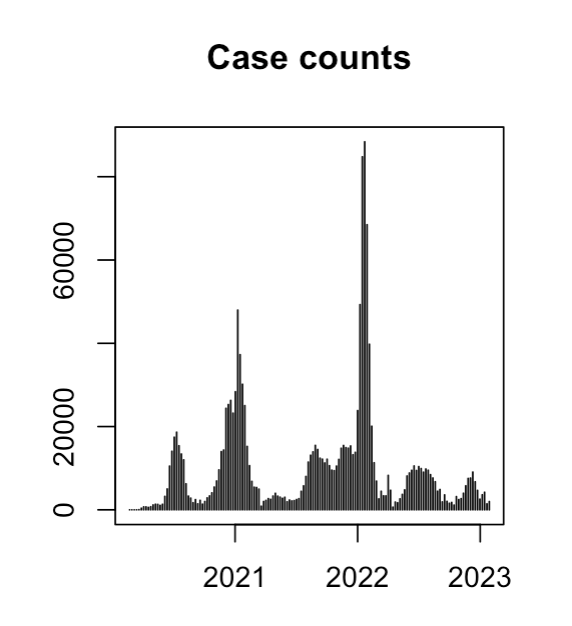
\includegraphics[height=4cm]{var}
\begin{itemize}[<+->] % using only the pause overlay specification
			\item Highly variable case count time series suggest transmission heterogeneity or changes in R
			\item Metrics of variability are overlooked: "How is variability related to different phases of an epidemic?"\cite{graham_measles_2019}
			\item Adam et al.\cite{adam_time-varying_2022} found that COVID-19 transmission heterogeneity decreased over time
	\end{itemize}
\end{frame}

\begin{frame}{\textbf{Why study variability?}}
    \begin{itemize}[<+->] % using only the pause overlay specification
		\item Dispersion of a case count time series may be a useful metric--part of a framework that models variance flexibly
		\item A 'mean crowding' parameter \cite{lloyd_mean_1967} was proposed: mean number per individual of other individuals in the same quadrat 
		\item Useful way to think about dispersion in case count time series, degree of dispersion is degree of clustering/crowding of cases
    \end{itemize}
		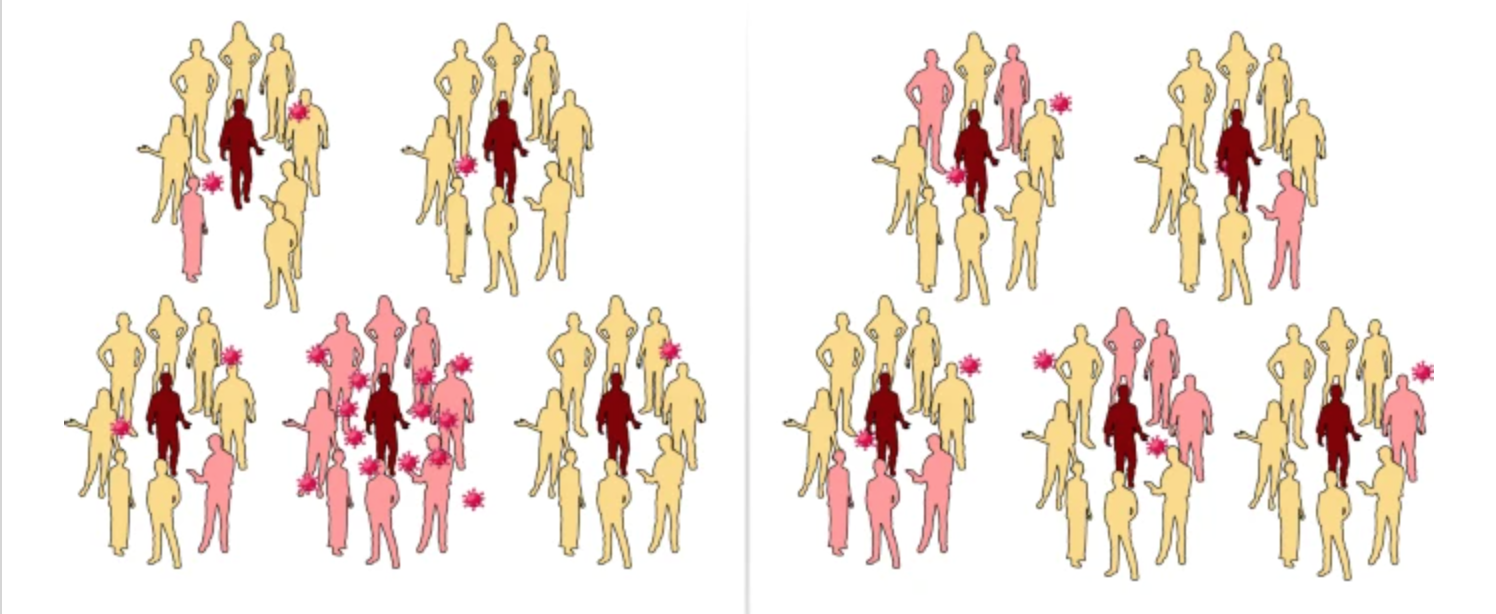
\includegraphics[height=2cm]{sup} \cite{nielsen_counterintuitive_2023}
\end{frame}

\section{Negative binomial model}
\begin{frame}{\textbf{Introduction to the method}}
    \begin{itemize}[<+->] % using only the pause overlay specification
		\item Let \begin{math}\lambda_t\end{math} be epidemic intensity at time t, I\begin{math}_t\end{math} be incidence at time t, and \begin{math}\theta_t\end{math} be dispersion at time t
		\item \begin{equation}\mathrm{I_t = NB(\mu = \lambda_t, \theta_t = I_{t-1})} 
		\end{equation} \cite{grenfell_dynamics_2002}
		\item Adjusted for population size using an offset in the model
		\item Linear predictor includes a natural spline in time to account for autocorrelation in case counts
		\begin{align}
			log(E[Y_i]/n_i) &= \beta_1h_1(t_i) + \beta_2h_2(t_i) + \beta_3h_3(t_i) \\
			log(E[Y_i])-log(n_i) &= \beta_1h_1(t_i) + \beta_2h_2(t_i) + \beta_3h_3(t_i) \\ 
			log(E[Y_i]) &= \beta_1h_1(t_i) + \beta_2h_2(t_i) + \beta_3h_3(t_i) + log(n_i) 
		\end{align}
            \item Model fit on a rolling basis to each time series
	\end{itemize}
\end{frame}

\begin{frame}{\textbf{Negative binomial model}}
\begin{itemize}[<+->] % using only the pause overlay specification
		\item 
            \begin{equation}
                f_t(I) = \binom{I + \theta - 1}{I} \left( \frac{\mu}{\mu+\theta} \right)^I \left( \frac{\theta}{\mu +\theta} \right)^\theta
            \end{equation}
		\item \begin{align}
		E(I) &= \mu\\
		Var(I) &= \mu + \frac{\mu^2}{\theta}
	\end{align}
	\item LRT framework: at each time step along a time series, fit null model and \begin{math}\theta\end{math} change model, conduct LRT to produce p-value
	\end{itemize}
\end{frame}

\begin{frame}{\textbf{Simulated time series data set}}
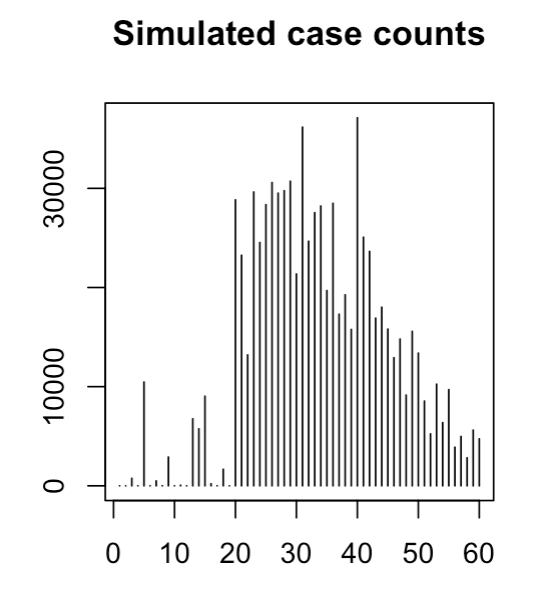
\includegraphics[height=3cm]{sim}
    \begin{itemize}[<+->] % using only the pause overlay specification
	\item Validity/power simulations: Gaussian and uniform epidemic curves with an attack rate of 0.1 
 	\item Varied magnitude of \begin{math}\theta\end{math} change, location of the change, underlying population size, and epidemic curve shape
	\item Epidemic curves over 60 time steps each were produced, and the LRT procedure was applied to each
\end{itemize}
\end{frame}

\begin{frame}{\textbf{Performance: simulated data}}
		\begin{figure}[!h]
			
\includegraphics[width=0.5\textwidth]{fig1}
			\caption{
				Detecting dispersion changes in incidence time series. A/B: Simulated incidence when dispersion is constant/changes. C/D: Constant/changing dispersion used above. E: Performance of LRT with simulated data that has different absolute differences in theta (x-axis of each pane) illustrates p-value distribution across different population sizes. O and X mark the null and alternative hypotheses indicated in panels C and D. 
			}
			\label{fig1}
		\end{figure}
\end{frame}

\begin{frame}{\textbf{Application to empirical data}}
    \begin{itemize}[<+->] % using only the pause overlay specification
            \item Weekly case counts from US counties between 2020-01-04 and 2023-03-18
		\item Estimated \begin{math}\theta_t\end{math} for 154 time steps for 144 US counties (IRLS procedure implemented via the NBPSeq package\cite{NBPSeq} and from Di et al.\cite{yanming_nbp_2011}) 
		\item Investigated large counties (largest three counties in each state)
	\end{itemize}
\end{frame}

\section{Results}
\begin{frame}{\textbf{}}
		\begin{figure}[!h]
			
\includegraphics[width=0.5\textwidth]{compare}
			\caption{
				Method applied to case counts between 2020-01-04 and 2023-03-18 for Jefferson County, AL. A: Case counts . B: LRT statistic C: Log dispersion parameter.
			}
			\label{fig2}
		\end{figure}
\end{frame}

\begin{frame}{\textbf{Results: empirical data}}
	\begin{figure}[!h]
	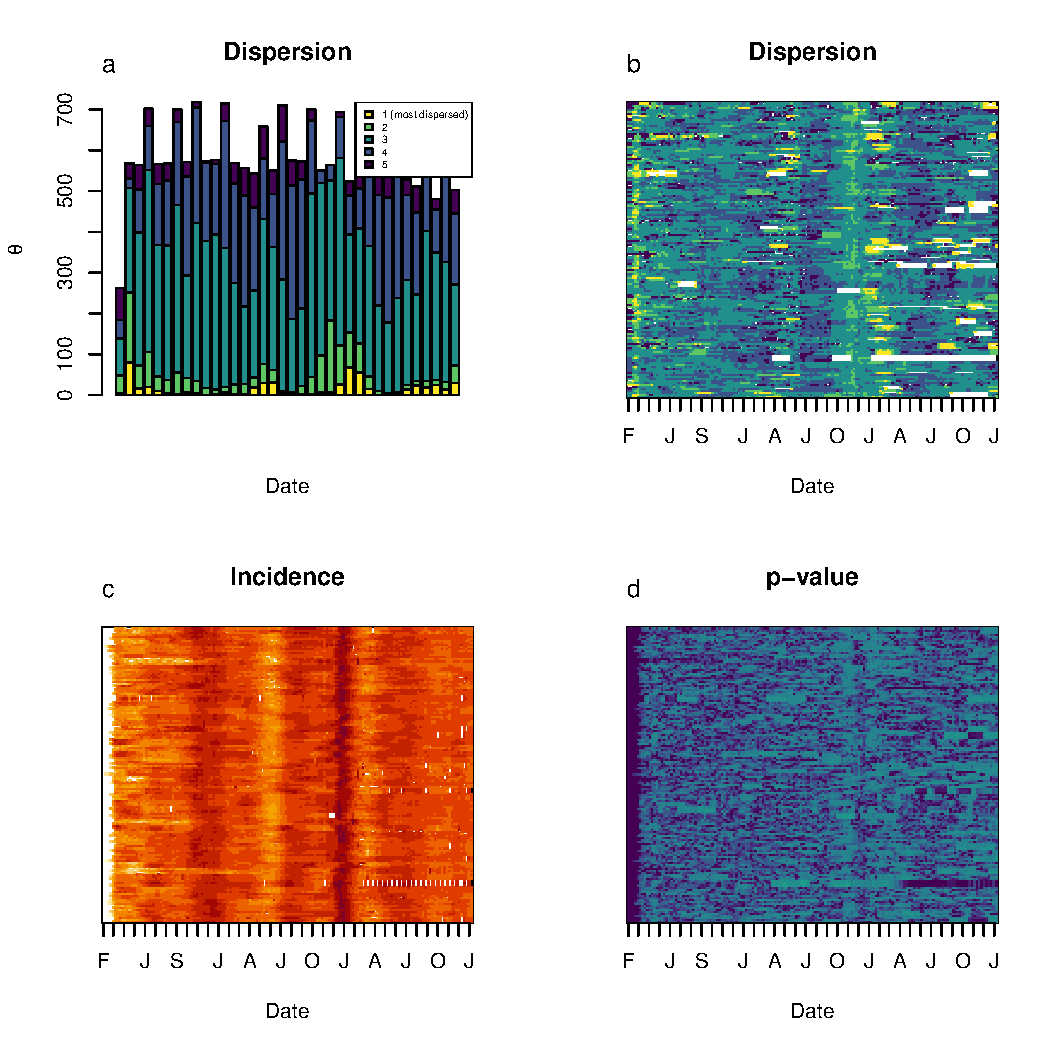
\includegraphics[width=0.5\textwidth]{fig2}
	\caption{
		Incidence and dispersion in large counties in the US. A: Binned log of the dispersion parameter. B: Log of the dispersion parameter for each of the large counties (y-axis). C: Log incidence for each of the large counties (y-axis). D: LRT p-values for each of the large counties (y-axis).
	}
	\label{fig2}
\end{figure}
\end{frame}

\section{Concluding remarks}
\begin{frame}{\textbf{Concluding remarks}}
    \begin{itemize}[<+->] % using only the pause overlay specification
            \item LRT procedure performed well for relevant range of population sizes
		\item Dispersion is high at unexpected times (near peak incidence)
            \item Concentration of changes in dispersion parameter near peak incidence
            \item Methods that use population-level data are important: timing/allocation of public health resources can be achieved with limited resources
	\end{itemize}
\end{frame}

\section{References}

\begin{frame}
{\tiny\printbibliography}
\end{frame}

\begin{frame}
	\begin{center}
		{\Huge Thanks!}
	\end{center}
\end{frame}

\end{document}